\section{Realizacja optymalizacji wybranej magistrali systemowej}
Ze względu na to, jak ważną odgrywają rolę magistrale w systemie mikrokomputerowym, w tym rozdziale zostanie przeanalizowana specyfikacja magistrali Wishbone oraz jej implementacja w systemie LiteX. Celem jest znalezienie części specyfikacji, które nie zostały zaimplementowane w LiteX, a które mogłyby przyspieszyć działanie systemu zbudowanego z jego wykorzystaniem.

\subsection{Budowa magistrali Wishbone}
Specyfikacja magistrali Wishbone definiuje wiele sygnałów, z których w praktyce wykorzystuje się wyłącznie część. W podstawowych zastosowaniach wykorzystywane są następujące sygnały, opisywane z perspektywy inicjatora (mastera):
\begin{itemize}
    \item szyna adresowa \texttt{ADR_O},
    \item szyny danych \texttt{DAT_I} oraz \texttt{DAT_O},
    \item sygnały synchronizacji \texttt{CYC_O}, \texttt{STB_O} oraz \texttt{ACK_I},
    \item sygnał odczytu/zapisu \texttt{WE_O},
    \item selektor bajtów słowa \texttt{SEL_O}
\end{itemize}

Szerokość szyn danych zależy od wielkości słowa, jakie mają być przesyłane w jednym cyklu zegara. Szerokość szyny adresowej zależy od tego, jaką przestrzeń adresową chcemy zaadresować. Magistrala wykorzystuje adresowanie po słowach --- jeśli pożądana jest operacja na mniejszej jednostce, np. bajcie, wykorzystywany jest sygnał \texttt{SEL_O} w celu wybrania fragmentu słowa na szynie danych, które druga strona może wykorzystać.

\subsection{Rodzaje cykli na szynie Wishbone}

\subsubsection{Wishbone Classic Bus Cycles}
Podstawowy rodzaj cykli na magistrali Wishbone obsługuje operacje odczytu lub zapisu pojedynczego słowa szyny w trakcie pojedynczego cyklu transferu.

Cykl rozpoczyna się poprzez asercję sygnału \texttt{CYC} przez inicjatora cyklu, a kończy poprzez jego negację. Sygnał \texttt{STB} zaś informuje o gotowości do transferu słowa i jest utrzymywany w stanie wysokim, dopóki jeden z sygnałów terminujących cykl (\texttt{ACK}, \texttt{ERR}, \texttt{RTY}) nie zostanie ustawiony w stan wysoki przez drugą stronę połączenia. Pozwala to na regulację prędkości transferu przez obie strony połączenia.

\begin{figure}[H]
    \centering
    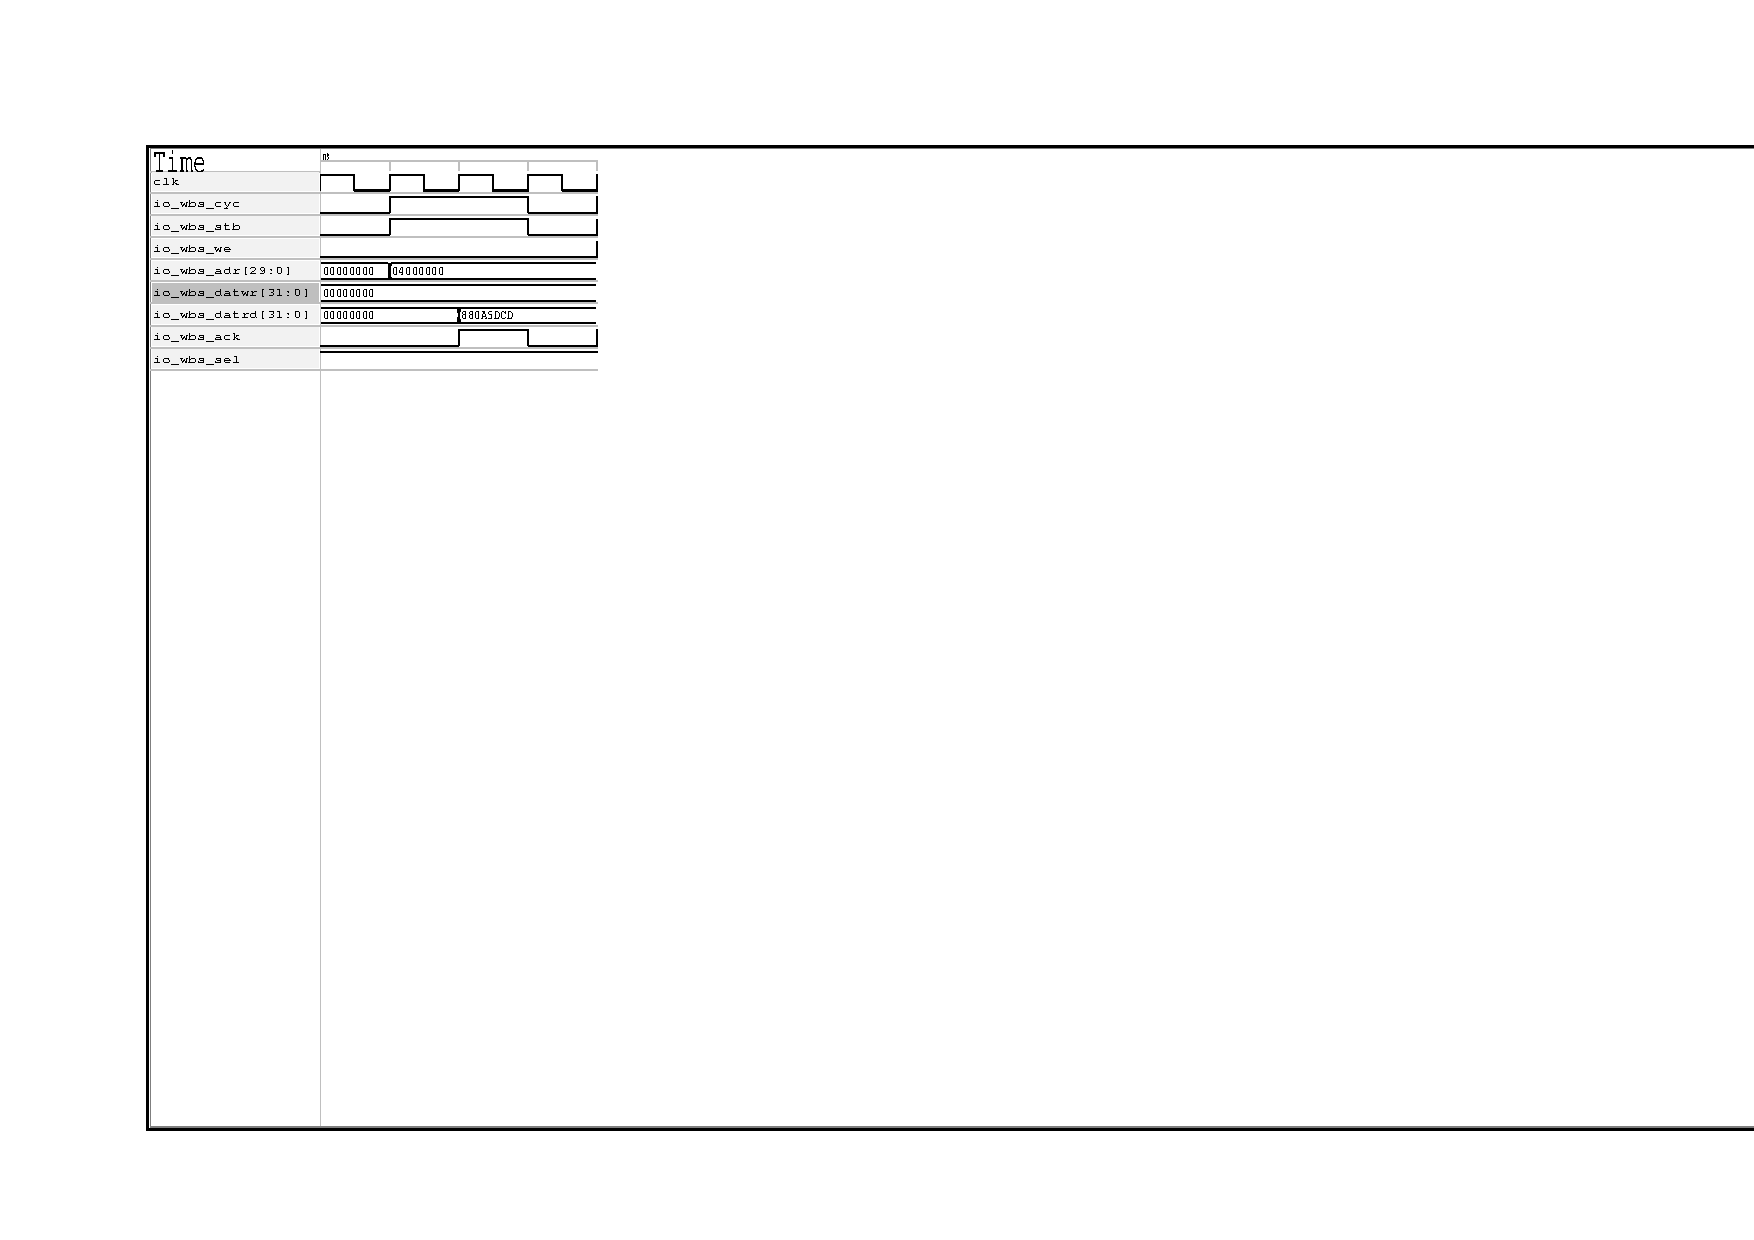
\includegraphics[scale=1.5,trim={2.54cm 14.73cm 19.6cm 2.9cm},clip]{implementation/classic-read.pdf}
    \caption{Przebieg pokazujący odczyt pojedynczego, 32-bitowego słowa po magistrali Wishbone}
    \label{fig:wishbone-classic-read}
\end{figure}

W celu transferu słowa wykorzystywane są przynajmniej następujące sygnały: linia adresowa (\texttt{ADR}), linia danych (\texttt{DAT_I}, \texttt{DAT_O}), linia wyboru fragmentu słowa (\texttt{SEL}) oraz sygnał kierunku operacji (\texttt{WE}). Strona inicjująca połączenie na początku cyklu wystawia adres, na którym ma być wykonywana operacja; słowo na szynie \texttt{DAT_O}, jeśli jest to operacja zapisu; linie wybierające, które części szyny danych będą wykorzystywane w transferze oraz kierunek operacji. W następnym takcie zegara druga strona może wystawić słowo na szynie wejściowej danych (\texttt{DAT_I}), jeśli jest to operacja zapisu, oraz ustawić w stan wysoki jeden z sygnałów synchronizujących --- \texttt{ACK}, który potwierdza realizację operacji; \texttt{ERR}, informujący o wystąpieniu błędu w trakcie transferu; oraz \texttt{RTY}, który informuje o chwilowej braku gotowości strony odbiorczej do obsługi transferu.

\begin{figure}[H]
    \centering
    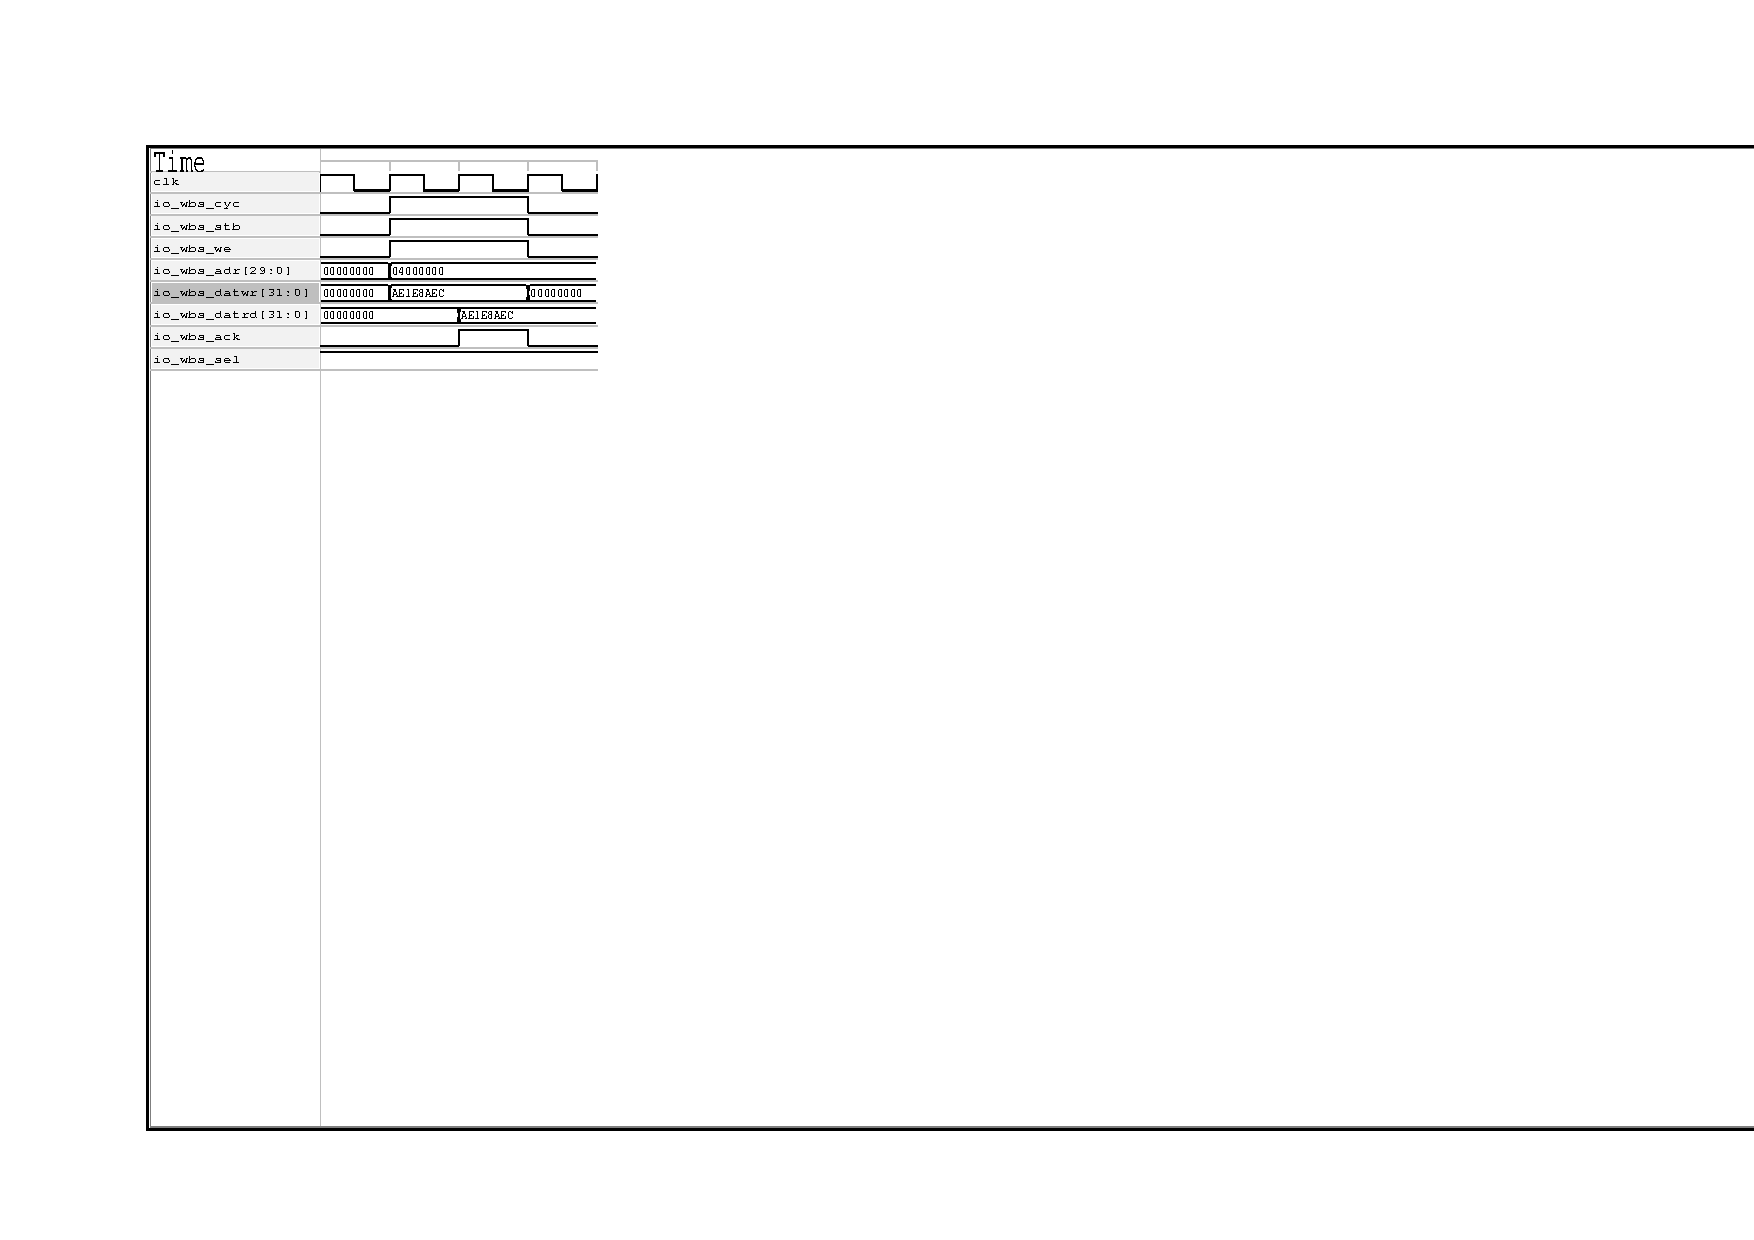
\includegraphics[scale=1.5,trim={2.54cm 14.73cm 19.6cm 2.9cm},clip]{implementation/classic-write.pdf}
    \caption{Przebieg pokazujący zapis pojedynczego, 32-bitowego słowa po magistrali Wishbone}
    \label{fig:wishbone-classic-write}
\end{figure}

W celu ograniczenia opóźnień przy transferze słów między kontrolerem a peryferium wykorzystuje się synchroniczne sygnały terminujące cykl. Wprowadza to jednak dodatkowe opóźnienie przy każdym słowie, gdyż peryferium nie jest świadome tego, że jest ponownie adresowane przy każdym kolejnym słowie --- z tego powodu po odebraniu lub wystawieniu słowa peryferium kończy cykl poprzez negację sygnału \texttt{ACK}. Oznacza to, że transfer każdego słowa w cyklu przypadają dwa takty zegara, zakładając, że peryferium nie potrzebuje dodatkowych opóźnień z innych powodów.

\begin{figure}[H]
    \centering
    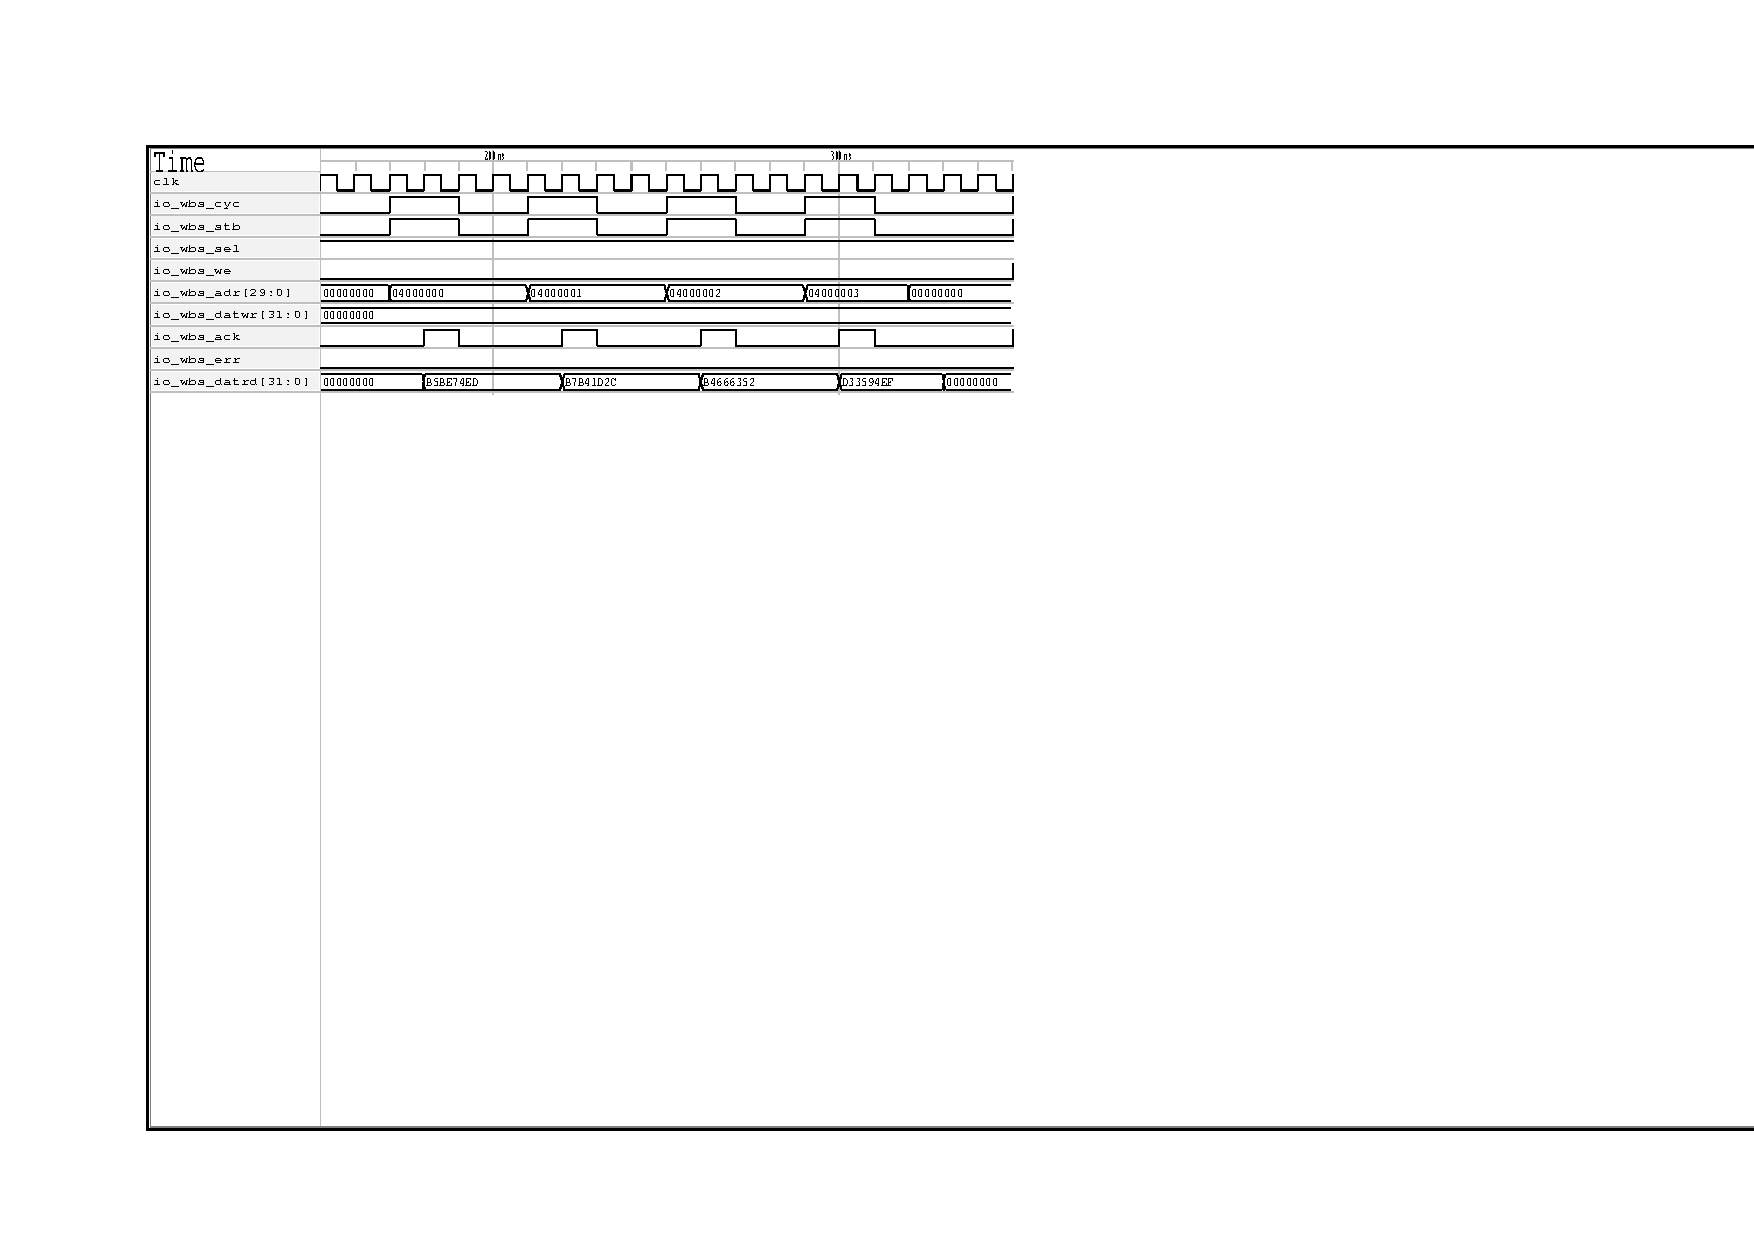
\includegraphics[scale=1,trim={2.54cm 14.37cm 13cm 2.9cm},clip]{implementation/classic-read-4.pdf}
    \caption{Przebieg pokazujący odczyt czterech 32-bitowych słów po magistrali Wishbone}
    \label{fig:wishbone-classic-read-4}
\end{figure}

\subsubsection{Wishbone Registered Feedback Bus Cycles}

Rozwiązaniem problemu cykli opóźniających przy transferze każdego kolejnego słowa jest rozbudowa magistrali o dodatkowe sygnały sterujące, które pozwoliłyby na informowanie peryferiów, że w danym cyklu magistrali nastąpi transfer większej ilości słów. Dzięki temu peryferium może się przygotować do odebrania większej ilości danych bez konieczności potwierdzania odbioru po każdym słowie.

Ten rodzaj synchronicznego terminowania cykli jest opisany w części specyfikacji "Wishbone Registered Feedback Bus Cycles". Dodaje ona dwa sygnały do magistrali, które są wykorzystywane do przekazywania informacji o rodzaju cyklu oraz związanego z nim dodatkowego parametru.

Sygnał \texttt{CTI} (Cycle Type Identifier) służy do identyfikowania rodzaju obecnie wykonywanego cyklu. Peryferium może wykorzystać tę informację, by przygotować się na kolejne części cyklu.
\begin{table}[H]
\begin{center}
\begin{tabular}{ r|l }
 CTI[2:0] & opis \\ 
 \hline
 0b000 & cykl klasyczny \\
 0b001 & cykl potokowy ze stałym adresem \\
 0b010 & cykl potokowy z inkrementacją adresu \\
 0b011 & zarezerwowane \\
 0b100 & zarezerwowane \\
 0b101 & zarezerwowane \\
 0b110 & zarezerwowane \\
 0b111 & zakończenie cyklu \\
 \hline
\end{tabular}
\end{center}
\caption{\label{tab:signal-states-cti}Rodzaje stanów sygnału \texttt{CTI}}
\end{table}

Sygnał \texttt{BTE} (Burst Type Extension) zawiera zaś dodatkowe informacje zależne od danego rodzaju aktualnego cyklu.
W obecnej wersji specyfikacji jest wykorzystywany tylko w cyklu potokowym z inkrementacją adresu; jego wartość dla tego rodzaju cyklu można interpretować w następujący sposób:

\begin{table}[H]
\begin{center}
\begin{tabular}{ r|l }
 BTE[1:0] & opis \\ 
 \hline
 0b00 & liniowa inkrementacja adresu \\
 0b01 & inkrementacja adresu z zawijaniem 2 najmniej znaczących bitów \\
 0b10 & inkrementacja adresu z zawijaniem 3 najmniej znaczących bitów \\
 0b11 & inkrementacja adresu z zawijaniem 4 najmniej znaczących bitów \\
 \hline
\end{tabular}
\end{center}
\caption{\label{tab:signal-states-bte}Rodzaje stanów sygnału \texttt{BTE} dla \texttt{CTI} równego \texttt{0b010}}
\end{table}

Cykle potokowe z zawijającą inkrementacją adresu są zwykle wykorzystywane przy wypełnianiu linii pamięci podręcznej (cache) procesora; pozwala to na pełne pokrycie linii pamięci podręcznej, gdy adres, od którego zaczyna się dany cykl potokowy, nie pokrywa się z szerokością linii pamięci cache (która mieści kilka słów transferowych, przez co adresowana jest z pominięciem kilku najmniej znaczących bitów adresu)
Cykle potokowe ze stałym adresem przydatne są zaś przy strumieniowaniu danych do konkretnego adresu pojedynczego peryferium (na przykład przetwornika cyfrowo-analogowego) poprzez wykorzystanie dedykowanego podzespołu do szybkich transferów danych, zwanych również z angielskiego Direct Memory Access.

\subsection{Implementacja podzespołu z obsługą cykli transmisji seryjnej do stałego adresu}

Pierwszą częścią projektu było stworzenie minimalnego peryferium, które oprócz interfejsu Wishbone ma również wyprowadzenia, które można wykorzystać w celu komunikacji z podzespołem drogą inną niż poprzez magistralę Wishbone. Głównym powodem jego powstania było zrozumienie działania interfejsu magistrali Wishbone w praktyce. Pozwoliłoby to również na weryfikację poprawności działania komunikacji poprzez porównywanie danych, które zostały zapisane lub odebrane z kontrolera poprzez magistralę z tymi, które można odebrać lub nadać do peryferium inną drogą.

\begin{figure}[H]
    \centering
    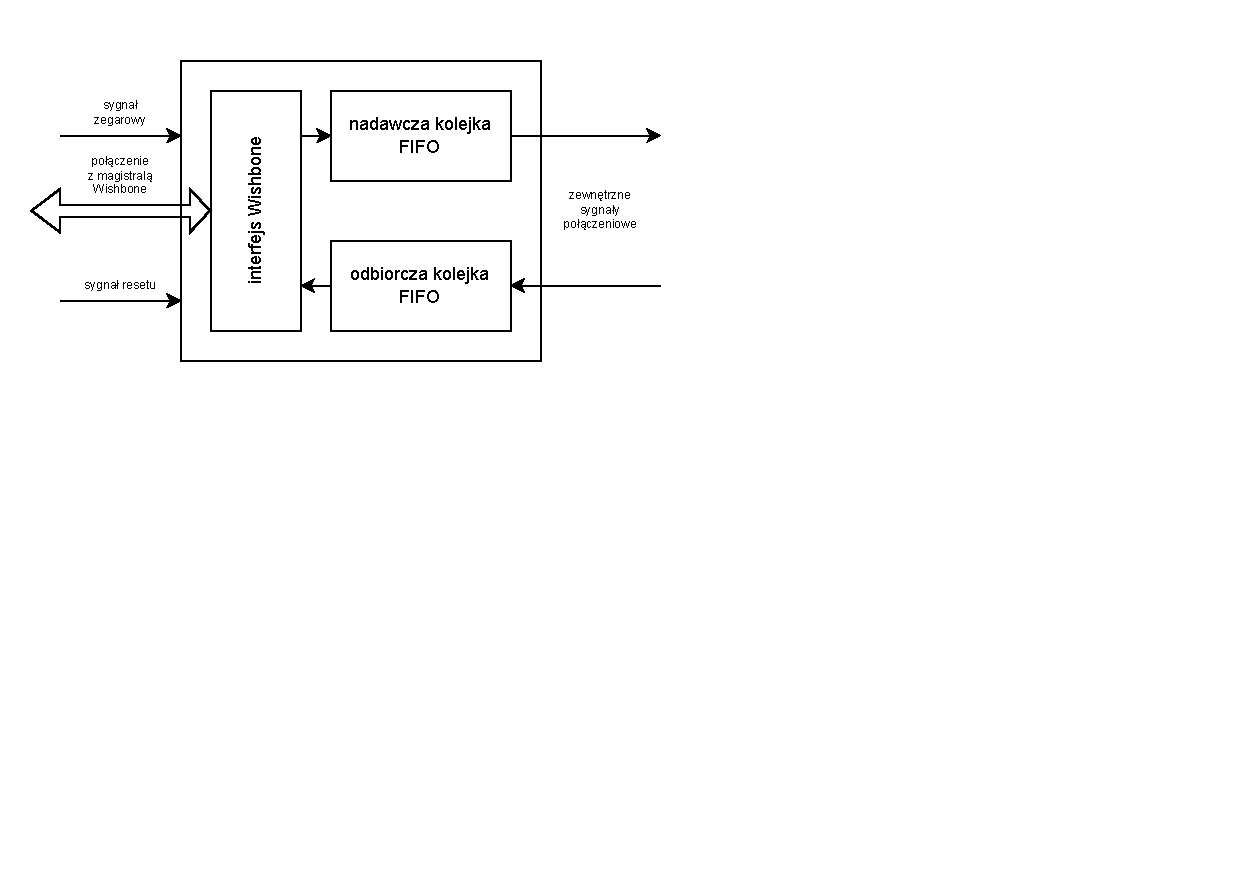
\includegraphics[scale=1,trim={0.5cm 8.5cm 9.5cm 1cm},clip]{implementation/fifo-peripheral-diag.pdf}
    \caption{Schemat blokowy przykładowego modułu komunikacyjnego wykorzystującego kolejki FIFO}
    \label{fig:fifo-peripheral-diag}
\end{figure}

Peryferium składa się z dwóch synchronicznych kolejek FIFO oraz logiki obsługującej magistralę Wishbone. Jedna kolejka FIFO służy do odbioru danych z zewnętrznego źródła, druga zaś odbiera dane z zewnętrznego źródła. Obie kolejki zostały podłączone do magistrali Wishbone z użyciem logiki zawierającej maszynę stanów skończonych, która zajmuje się sterowaniem sygnałami synchronizacji portów wewnętrznych kolejek w zależności od rodzaju operacji na magistrali (odczyt lub zapis). Zewnętrzne porty kolejek zostały wyprowadzone na zewnątrz peryferium bez dodatkowej logiki sterującej w celu ułatwienia przeprowadzenia testów na dalszych etapach pracy. Kolejki są dostępne jako gotowy element w module \texttt{migen.genlib} będącej częścią biblioteki do opisu logiki Migen.

\begin{figure}[H]
    \centering
    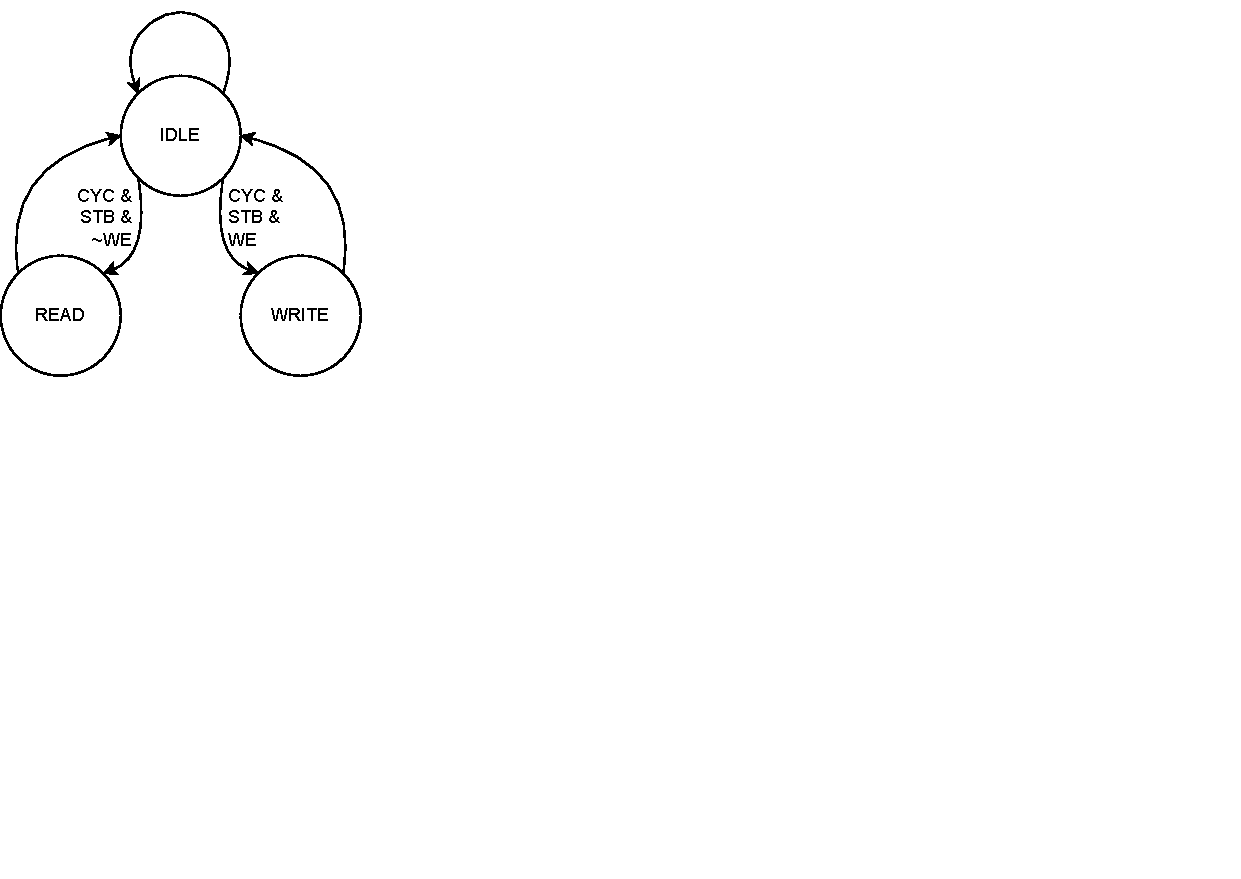
\includegraphics[scale=1,trim={0 8.5cm 14.8cm 0.1cm},clip]{implementation/fifo-fsm-orig.pdf}
    \caption{Graf maszyny stanowej interfejsu Wishbone będącego częścią modułu transmisyjnego FIFO}
    \label{fig:fifo-fsm-orig}
\end{figure}

Maszyna stanowa składa się z trzech stanów: \texttt{IDLE}, \texttt{READ} oraz \texttt{WRITE}.
Stanem startowym jest \texttt{IDLE}. Gdy zostanie zainicjowany cykl transferu danych na magistrali poprzez ustalenie stanu wysokiego sygnałów \texttt{CYC} oraz \texttt{STB}, maszyna w kolejnym takcie zegara przejdzie do stanu \texttt{READ} lub \texttt{WRITE}, w zależności od stanu sygnału WE na magistrali.
Przy stanie \texttt{WRITE} sprawdzany jest stan sygnału \texttt{writable} na wewnętrznym porcie wyjściowej kolejki FIFO. Jeśli kolejka nie jest zapełniona, są ustalenie stanu wysokiego sygnały: \texttt{WE} portu zapisu kolejki, powodujący zapisanie słowa wystawionego na magistrali do kolejki oraz \texttt{ACK} magistrali, który służy do informowania kontrolera szyny, że transmisja została potwierdzona. W przypadku, gdy kolejka jest zapełniona, sygnały \texttt{ACK} magistrali oraz \texttt{WE} kolejki nadawczej są negowane --- w ten sposób kontroler magistrali wie, że peryferium nie może potwierdzić przetworzenia odebranego słowa.
Podobnie funkcjonuje to przy stanie \texttt{READ} maszyny, jednak w tym wypadku potwierdzenie transmisji zależy od tego, czy w kolejce znajduje się przynajmniej jedno słowo, które można odczytać z kolejki --- o obecności danych w kolejce informuje sygnał \texttt{readable} kolejki odbiorczej, zaś potwierdzenie odczytania słowa w kolejce jest potwierdzane poprzez ustalenie stanu wysokiego sygnału \texttt{RE} kolejki odbiorczej.

Z reguły 4.35 opisanej w specyfikacji magistrali Wishbone wynika fakt, że w trakcie trwania cyklu potokowego ze stałym adresem nie mogą zmienić się następujące sygnały magistrali: linia adresowa, linia wybierająca \texttt{SEL} oraz wybór operacji \texttt{WE}. Wobec tego można założyć, że cykl rozpoczęty operacją zapisu będzie w kolejnych taktach zegara przekazywał kolejne słowa do odebrania przez podzespół.

\begin{figure}[H]
    \centering
    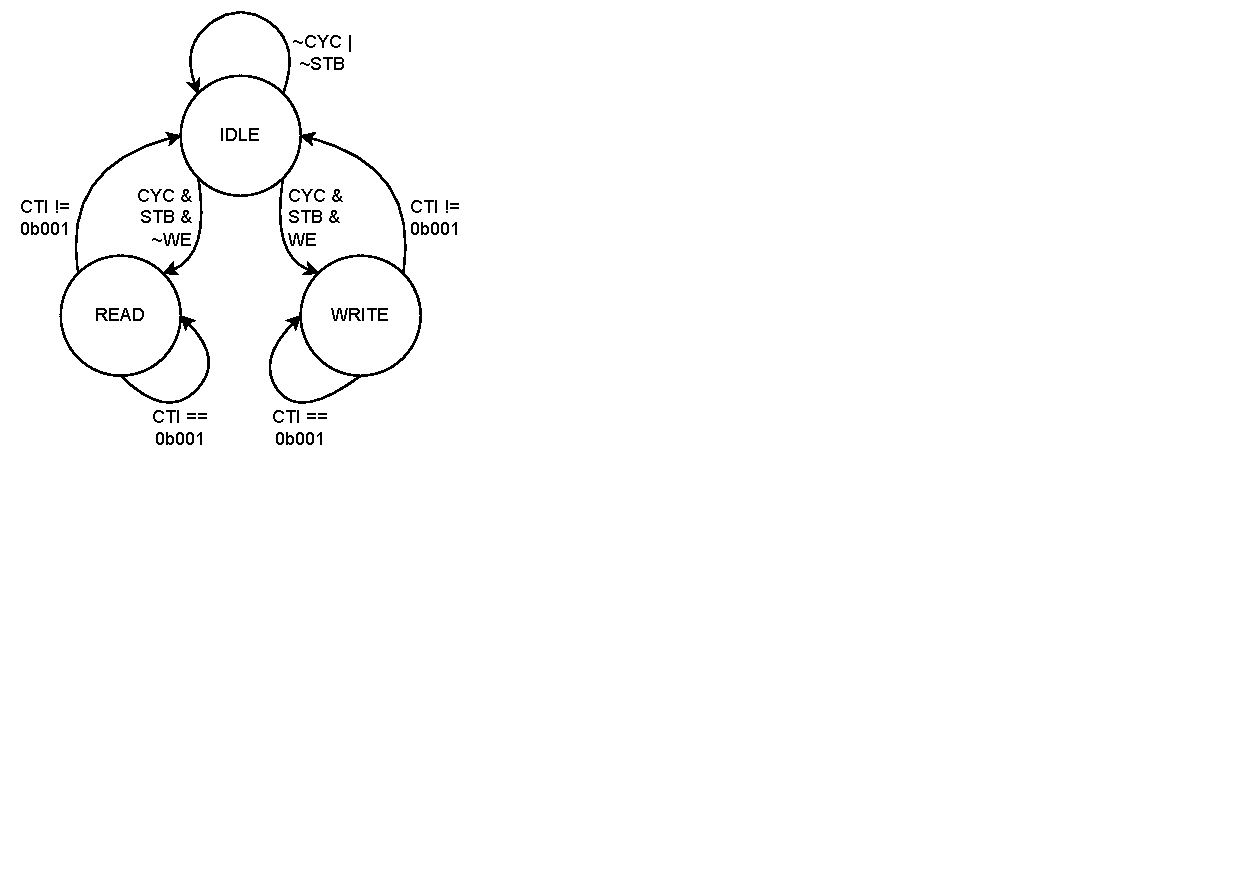
\includegraphics[scale=1,trim={0 7cm 13cm 0.1cm},clip]{implementation/fifo-fsm-burst.pdf}
    \caption{Graf maszyny stanowej interfejsu Wishbone modułu transmisyjnego z dodaną obsługą transferu potokowego}
    \label{fig:fifo-fsm-burst}
\end{figure}

W celu kontynuowania cyklu przy każdym takcie zegara sprawdzane są następujące warunki: czy cykl dalej jest aktywny (sygnały \texttt{CYC} i \texttt{STB} są aktywne) oraz czy sygnał przekazujący rodzaj cyklu \texttt{CTI} ma dalej wartość \texttt{0b001}, oznaczający cykl potokowy ze stałym adresem. Jeśli oba te warunki są spełnione, to ponawiamy obecny stan maszyny stanów w następnym takcie zegara, podtrzymując sygnał \texttt{ACK} w stanie wysokim. Dzięki temu w każdym takcie zegara kolejne słowa zostaną odebrane z kolejki odbiorczej albo dodane do kolejki nadawczej w podzespole, bez rozpoczynania nowego cyklu magistrali.

\subsection{Rozbudowanie istniejącego podzespołu (SRAM) o obsługę cykli transmisji seryjnej z inkrementacją adresu}

Peryferium SRAM, będący częścią biblioteki rdzeni w środowisku LiteX, składa się z dwóch części: synchronicznej pamięci (z biblioteki Migen) o zdefiniowanej szerokości słowa i pojemności (liczonej w słowach) oraz z interfejsu Wishbone, który łączy wspomnianą pamięć z magistralą.

\begin{figure}[H]
    \centering
    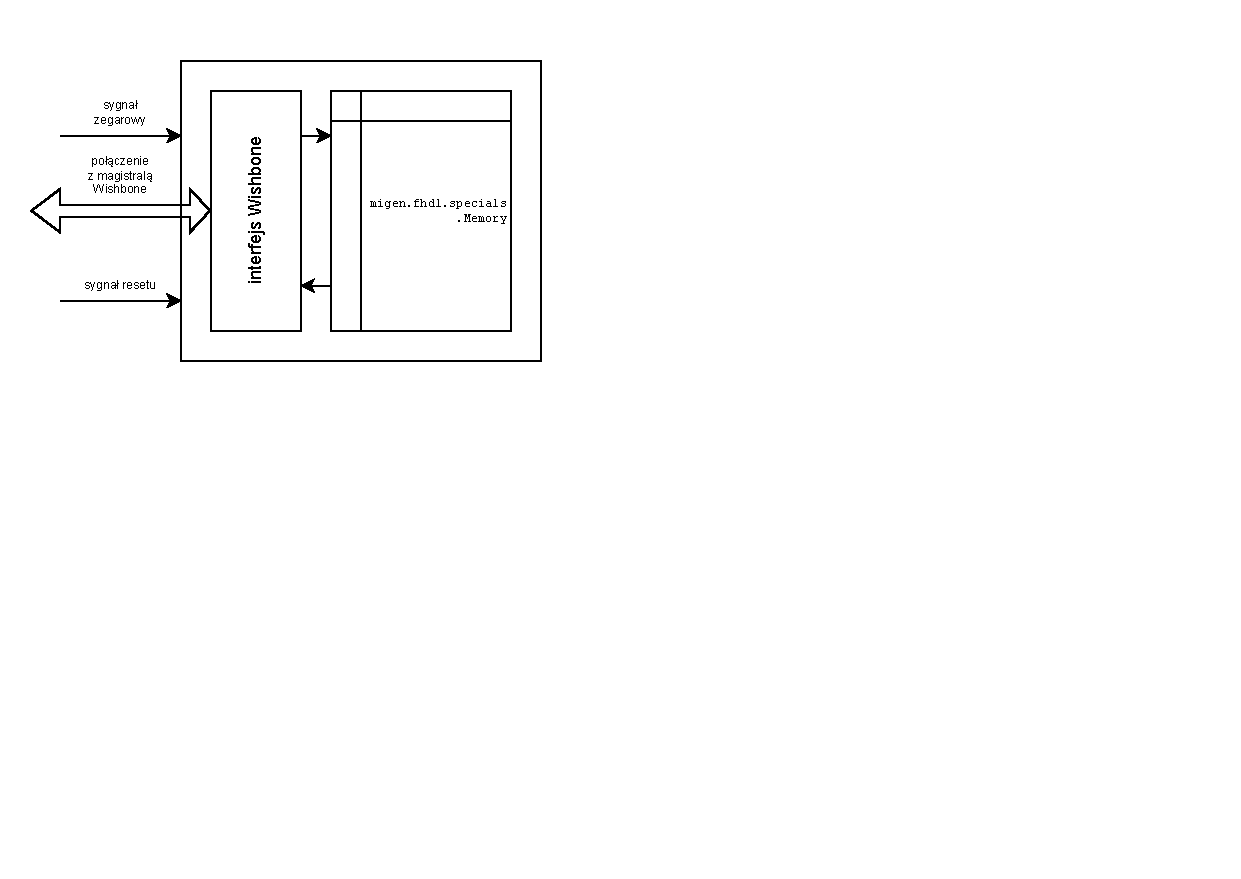
\includegraphics[scale=1,trim={0.5cm 8.5cm 9.5cm 1cm},clip]{implementation/memory-peripheral-diag.pdf}
    \caption{Schemat blokowy modułu SRAM z biblioteki peryferiów LiteX}
    \label{fig:memory-peripheral-diag}
\end{figure}

Interfejs implementuje wyłącznie podstawowy rodzaj cykli --- jako, iż wybrany procesor obsługuje potokowe transfery danych, będziemy w stanie, po rozbudowaniu implementacji interfejsu w module SRAM, zweryfikować wpływ obsługi transferów potokowych na praktyczną wydajność systemu mikroprocesorowego.

W celu dodania obsługi transferów potokowych do modułu SRAM, należy rozbudować interfejs o następujące elementy: generator adresów, wykorzystywany do wyznaczania kolejnych adresów pamięci w każdym cyklu zegara; dodatkowy warunek w logice kombinacyjnej odpowiedzialnej za generowanie sygnału potwierdzenia \texttt{ACK}; logika przekazywania wyznaczonych adresów.

Zakładamy, że wewnętrzny moduł pamięci RAM jest w stanie wykonywać kolejne operacje w każdym takcie zegara, tj. w każdym takcie zegara można wykonać operację odczytu lub zapisu słowa pod dowolnym adresem.
Kolejnym założeniem, wynikającym ze specyfikacji magistrali, jest niezmienność sygnałów \texttt{CTI} oraz \texttt{BTE} informujących o rodzaju cyklu w czasie jego trwania, z wyłączeniem stanu sygnału \texttt{CTI} informującym o zakończeniu cyklu potokowego.

\subsubsection{Detekcja rodzaju cyklu}

Strona inicjująca połączenie informuje o rodzaju cyklu poprzez sygnał \texttt{CTI}. Jeśli jedna ze stron transferu nie obsługuje wybranego typu cyklu, wtedy transfer przebiega jak w cyklu klasycznym (jeden transfer --- jeden cykl).
Z dwóch zdefiniowanych w specyfikacji rodzajów cykli potokowych, ze stałym adresem oraz inkrementacją adresu, w przypadku pamięci RAM interesuje nas cykl potokowy z inkrementacją adresu. W tym celu wykorzystamy warunek kombinacyjny, który w wypadku wystąpienia wspieranego rodzaju cyklu sygnalizuje żądanie transferu potokowego.
Oprócz tego definiujemy wektor \texttt{adr_counter_base}, w którym będzie zawarty adres bazowy z wyłączeniem bitów, które będą wykorzystywane w przypadku inkrementacji adresu z zapętleniem najmniej znaczących bitów.

\begin{listing}[H]
\begin{minted}{python}
class SRAM(Module):
    def __init__(self, mem_or_size, read_only=None, init=None, bus=None, burst=True):
            # ...
            adr_burst = Signal()

            # Obsługiwane są tylko cykle z inkrementacją adresu
            self.comb += [
                Case(self.bus.cti, {
                    # cykl z inkrementacją adresu
                    0b010: adr_burst.eq(1),
                    # zakończenie cyklu
                    0b111: adr_burst.eq(0),
                    # pozostałe rodzaje cykli (w tym cykl standardowy)
                    "default": adr_burst.eq(0)
                }),
            ]
\end{minted}
\caption{Logika kombinacyjna generująca sygnał informujący o cyklu potokowym na podstawie sygnału \texttt{CTI}}
\label{lst:impl-sram-detect}
\end{listing}

\subsubsection{Generator sekwencji adresów}

Gdy cykl zostanie rozpoczęty poprzez obecność stanu wysokiego sygnałów \texttt{CYC} i \texttt{STB} oraz inicjator połączenia zażąda transferu potokowego, inicjalizowany jest licznik adresów. Jest on wykorzystywany do generowania kolejnych adresów, do których dostęp strona inicjalizująca połączenie chce mieć dostęp w kolejnych taktach zegara bez oczekiwania na podanie kolejnych adresów. Gdy adres został zapisany w liczniku, w kolejnych taktach zegara licznik będzie inkrementowany o 1.
Jednocześnie w dodatkowym rejestrze, nazwanym \texttt{adr_counter_offset} zapisywane są dolne bity pierwszego zażądanego adresu. Zawartość tego dodatkowego rejestru będzie wykorzystywana do wyliczenia dolnych bitów dolnego adresu, jeśli inkrementacja adresu ma następować z zawijaniem dolnych bitów.

\begin{longlisting}
\begin{minted}{python}
class SRAM(Module):
    def __init__(self, mem_or_size, read_only=None, init=None, bus=None, burst=True):
        # ...
        adr_wrap_mask = Array((0b0000, 0b0011, 0b0111, 0b1111))
        adr_wrap_max = adr_wrap_mask[-1].bit_length()

        adr_latched = Signal()

        adr_counter = Signal(len(self.bus.adr))
        adr_counter_offset = Signal(adr_wrap_max)

        # Zapisanie adresu startowego nowego cyklu
        self.sync += [
            If(self.bus.cyc & self.bus.stb & adr_burst,
                adr_latched.eq(1),
                # Jeśli adres został zapisany, inkrementuj go w każdym takcie zegara
                If(adr_latched,
                    adr_counter.eq(adr_counter + 1)
                ).Else(
                    # Zapisz najmniej znaczące bity adresu w wypadku cyklu
                    # z zawijaniem adresu
                    adr_counter_offset.eq(self.bus.adr & adr_wrap_mask[self.bus.bte]),
                    # Zapisz adres bez najmniej znaczących bitów,
                    # jeśli trwa cykl z zawijaniem adresu. Jeśli będzie to operacja odczytu,
                    # licznik będzie preinkrementowany o 1
                    If(self.bus.we,
                        adr_counter.eq(
                            Cat(self.bus.adr & ~adr_wrap_mask[self.bus.bte],
                                self.bus.adr[adr_wrap_max:]
                                )
                        ),
                    ).Else(
                        adr_counter.eq(
                            Cat(self.bus.adr & ~adr_wrap_mask[self.bus.bte],
                                self.bus.adr[adr_wrap_max:]
                                ) + 1
                        ),
                    )
                ),
                If(self.bus.cti == 0b111,
                    adr_latched.eq(0),
                    adr_counter.eq(0),
                    adr_counter_offset.eq(0)
                )
            # Zerowanie licznika po zakończeniu cyklu
            ).Else(
                adr_latched.eq(0),
                adr_counter.eq(0),
                adr_counter_offset.eq(0)
            ),
        ]
\end{minted}
\caption{Fragment logiki synchronicznej odpowiedzialnej za kontrolę licznika adresu}
\label{lst:impl-sram-adrcounter}
\end{longlisting}

Gdy inicjator cyklu informuje o zakończeniu transferu potokowego poprzez ustawienie odpowiedniej wartości na sygnale \texttt{CTI}, licznik jest zerowany i zatrzymywany, by przy kolejnych taktach zegara nie wykonywać nadmiarowych operacji w pamięci.

W części kombinacyjnej generatora następny adres jest wyznaczany poprzez zsumowanie dwóch sygnałów, gdzie jeden sygnał zawiera wartość licznika bez zawijanych bitów adresu, natomiast drugi sygnał zawiera dolne bity adresu wyznaczone poprzez zsumowanie zawartości licznika i rejestru zawierającego dolne bity adresu początkowego, z których wykorzystywane są wyłącznie zawinięte bity.

\begin{listing}[H]
\begin{minted}{python}
class SRAM(Module):
    def __init__(self, mem_or_size, read_only=None, init=None, bus=None, burst=True):
        # ...
        adr_offset_lsb = Signal(adr_wrap_max)
        adr_offset_msb = Signal(len(self.bus.adr))
        adr_next = Signal(len(self.bus.adr))

        # Wyznacz kolejny adres poprzez zsumowanie zawartości licznika
        # z przesunięciem wyznaczonym przez najmniej znaczące bity adresu startowego
        self.comb += [
            adr_offset_lsb.eq((adr_counter + adr_counter_offset) & adr_wrap_mask[self.bus.bte]),
            adr_offset_msb.eq(adr_counter & ~adr_wrap_mask[self.bus.bte]),
            adr_next.eq(adr_offset_msb + adr_offset_lsb)
        ]
\end{minted}
\caption{Logika kombinacyjna odpowiedzialna za sumowanie docelowego adresu w każdym cyklu zegara}
\label{lst:impl-sram-adrnext}
\end{listing}

Wyznaczany adres, jeśli licznik jest uruchomiony, jest przekazywany w logice kombinacyjnej do linii adresowej modułu pamięci RAM --- w przeciwnym wypadku adres do pamięci RAM jest przekazywany bezpośrednio z magistrali, wliczając pierwszy adres przy transferach potokowych.

\subsubsection{Generowanie sygnału potwierdzenia}

Logika synchroniczna odpowiedzialna za generowanie sygnału \texttt{ACK} została zmodyfikowana w nieznaczny sposób, poprzez dodanie warunku OR dla zanegowanego sygnału \texttt{ACK} z poprzedniego taktu oraz wewnętrznego sygnału informującego o aktywnym transferze potokowym. W ten sposób sygnał \texttt{ACK} jest aktywny w każdym takcie zegara przy transferach potokowych, przy klasycznych cyklach zaś zachowanie jest to samo co poprzednio, czyli sygnał \texttt{ACK} jest natychmiastowo negowany w drugim takcie zegara po rozpoczęciu transferu.

\begin{listing}[H]
\begin{minted}{python}
class SRAM(Module):
    def __init__(self, mem_or_size, read_only=None, init=None, bus=None, burst=True):
        # ...
        self.sync += [
            self.bus.ack.eq(0),
            If(self.bus.cyc & self.bus.stb & (~self.bus.ack | adr_burst),
                self.bus.ack.eq(1)
            )
        ]
\end{minted}
\caption{Fragment logiki synchronicznej generującej sygnał ACK}
\label{lst:impl-sram-ack}
\end{listing}

W celu uproszczenia kodu sygnał \texttt{adr_burst} jest zawsze generowany w układzie, nawet jeśli obsługa transferów potokowych zostanie wyłączana --- w tym wypadku sygnał ten ma zawsze wartość \texttt{0b0}; sygnał ten może zostać automatycznie usunięty w trakcie optymalizacji układu przez programy do syntezy logiki.

\subsection{Wnioski po zaimplementowaniu optymalizacji wybranego peryferium}

Omówiona została magistrala Wishbone, bazując zarówno na specyfikacji, jak i przykładowej implementacji zawartej w projekcie LiteX.
Na potrzeby dalszych działań przedstawione zostały: moduł pamięci SRAM oraz moduł transmisyjny zbudowany z dwóch kolejek FIFO. Pozwoliło to na zademonstrowanie sposobu implementacji wybranej optymalizacji, czyli transferów potokowych, w istniejących modułach.
Dzięki prostocie implementacji interfejsu magistrali w module pamięci SRAM, jak i samego modułu wprowadzenie obsługi transferów potokowych nie wymagało większych zmian w logice interfejsu --- całość została sprowadzona do zaimplementowania licznika adresu po stronie modułu oraz dodatkowych warunków w logice synchronizującej komunikację po magistrali Wishbone.
